% Chapter Template

\chapter{IoT Healthcare} % Main chapter title

\label{IoT Healthcare} % Change X to a consecutive number; for referencing this chapter elsewhere, use \ref{ChapterX}

%----------------------------------------------------------------------------------------
%	SECTION 1
%----------------------------------------------------------------------------------------

\section{About the application}

This application is a prof of concept for a healthcare 

\subsection{Views}

\subsubsection{Smart Bands}
Here you can manage the smart bands registered in this platform and also add new bands.
\begin{figure}[h!]
	\centering
	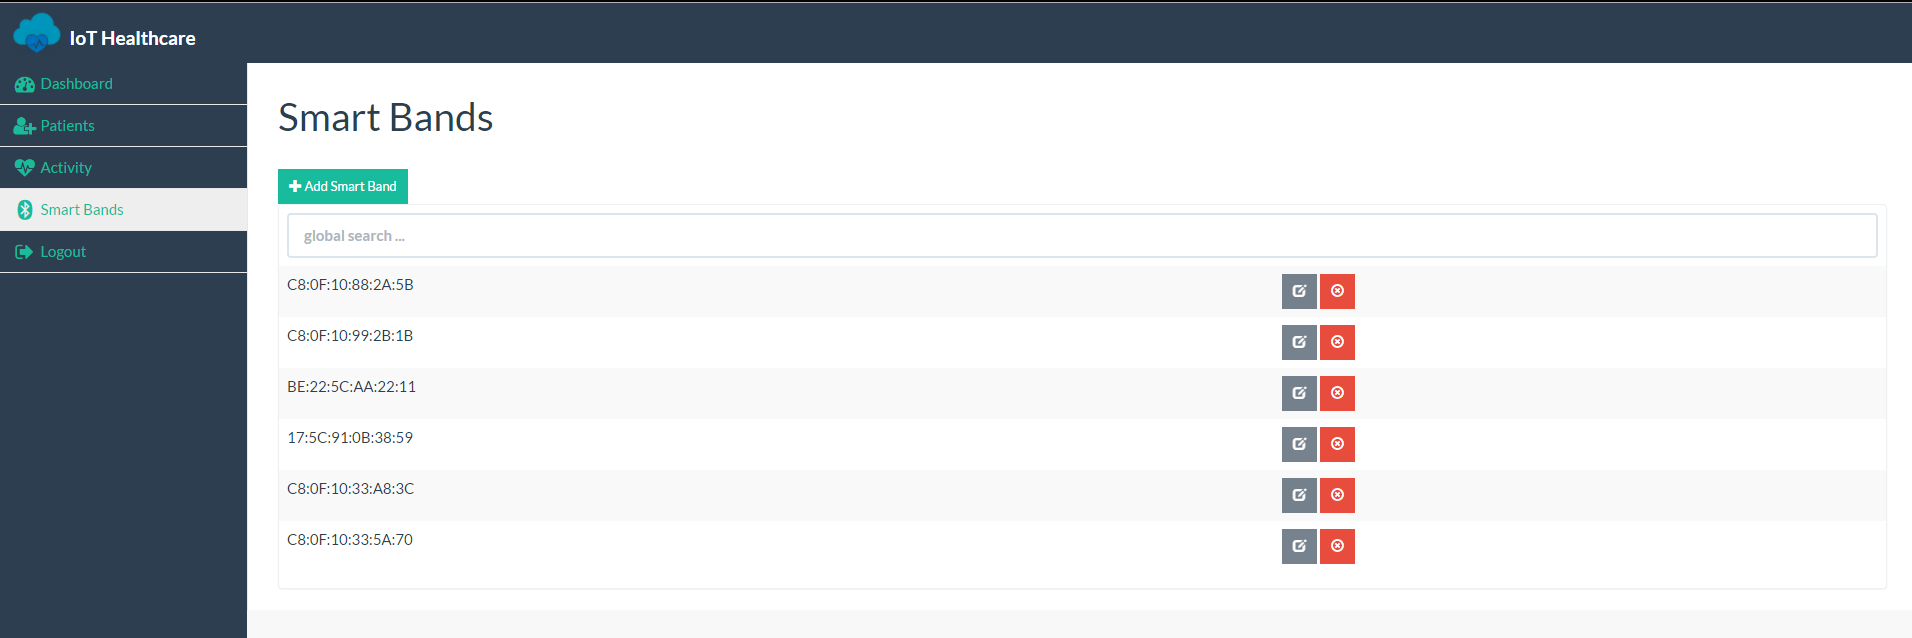
\includegraphics[width=1\textwidth]{./images/iothsmartbands}
	\rule{1\textwidth}{1pt}
	\caption{IoT Healthcare smartbands page}
\end{figure}


\subsubsection{Patients}
In the patients page you can manage all the patients each patient can have linked a smartband.

\begin{figure}[h!]
	\centering
	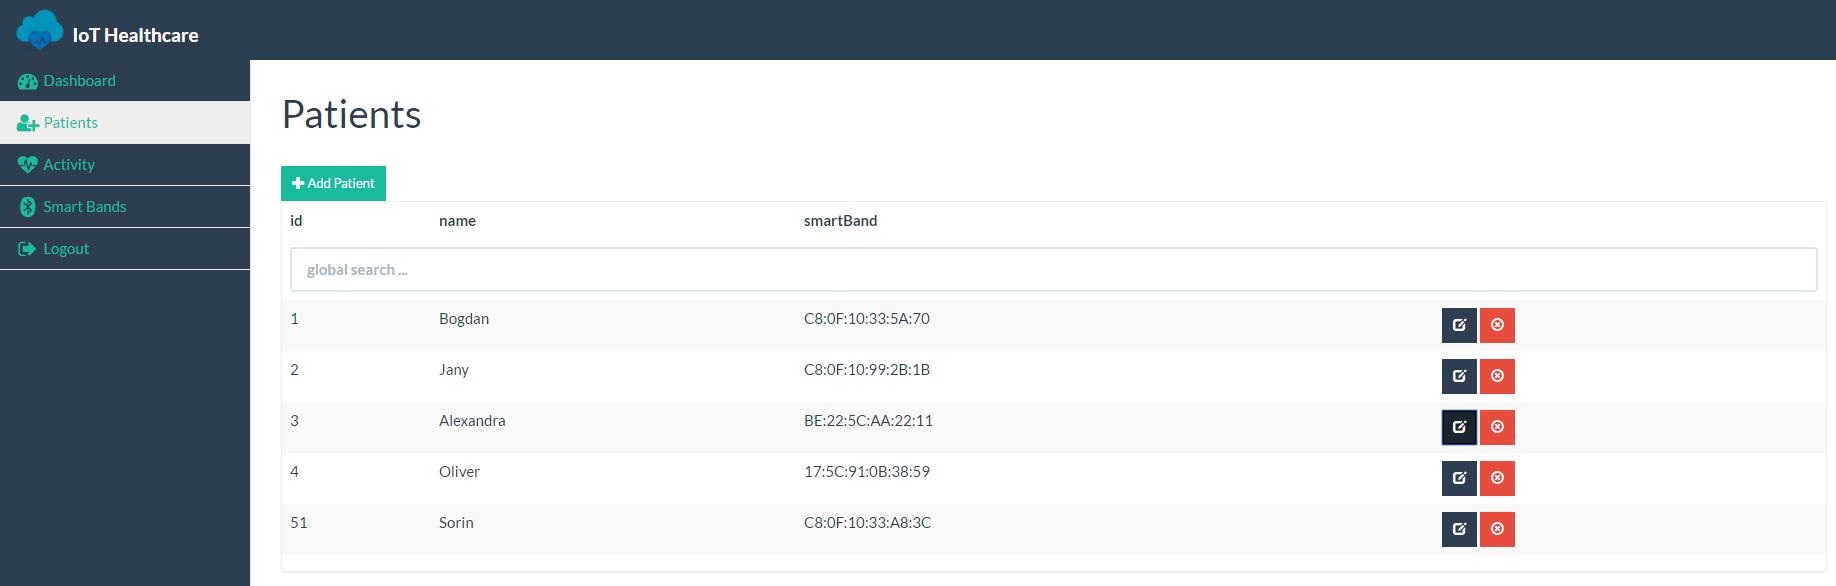
\includegraphics[width=1\textwidth]{./images/iothpatient}
	\rule{1\textwidth}{1pt}
	\caption{IoT Healthcare patients page}
\end{figure}

\subsubsection{Activity}
In the activity tab here is where the magic is happening. The daemon is sending an activity record every 20 min for each patient the record object has the number steps, an array of the heart rate values, the mac address of the smartband and of course the timestamp. 
\begin{lstlisting}[language=Bash] 
{
	"steps": 500,
	"heartRate": [
		43,
		89,
		30,
		40,
		0,
		5
	],
	"smartBand": {
		"mac": "C8:0F:10:88:2A:5B"
	},
	"timestamp": 1492617449907   
}
\end{lstlisting}      

\begin{figure}[h!]
	\centering
	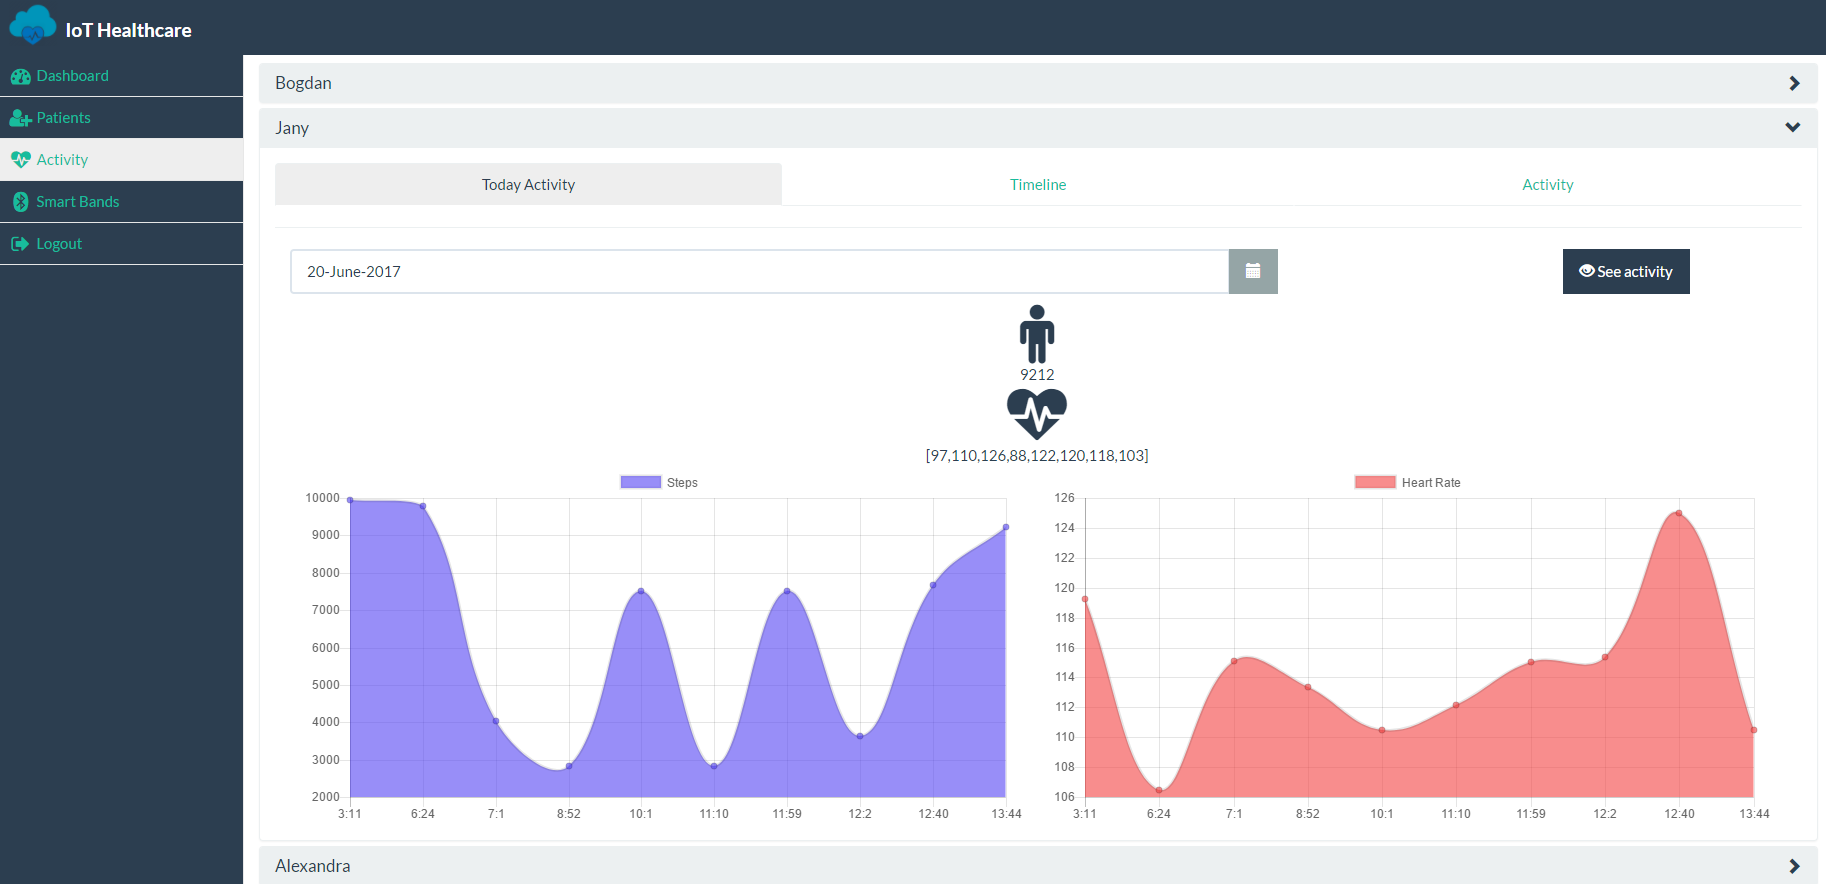
\includegraphics[width=1\textwidth]{./images/iothactivity}
	\rule{1\textwidth}{1pt}
	\caption{IoT Healthcare activity page}
\end{figure}
